\documentclass[whitelogo,oneside]{TUD-report2020}
\setcounter{secnumdepth}{3}
\usepackage{hyperref}
\usepackage{xcolor}
\usepackage{soul}
\usepackage{biblatex}
\addbibresource{report.bib}
\usepackage{multicol}
\usepackage{csquotes}
\usepackage{parskip}




\usepackage{longtable}
\usepackage{makecell}

\usepackage{changes}


\usepackage{graphicx}
\usepackage[justification=centering]{caption}

%For VHDL code
\usepackage{listings}      % For typesetting code
\usepackage{xcolor}        % For custom colors
\usepackage{courier}       % For a monospaced font









\begin{document}


%% for VHDL code
\lstdefinestyle{vhdlStyle}{
    language=VHDL,
    basicstyle=\footnotesize\ttfamily,
    keywordstyle=\color{blue},
    commentstyle=\color{green!40!black},
    stringstyle=\color{orange},
    showstringspaces=false,
    morekeywords={library,use,all,entity,is,port,in,out,end,architecture,of,begin,and,or,not,if,then,else,elsif,when,case,with,select,others,signal}
}

% Customized VHDL code environment
\newenvironment{vhdlcode}
{\lstset{style=vhdlStyle}}
{}

%% Use Roman numerals for the page numbers of the title pages and table of
%% contents.
\frontmatter

%% Uncomment following 19 lines for a cover with a picture on the lower half only
\title[tudelft-black]{\Huge{EPO 2 Final Report}}

\author[tudelft-white]{\Large{
Chantal Chen \\ 
Thijs van Esch \\ 
Eojin Lim \\ 
Pieter Olyslaegers \\
Kevin Pang \\ 
Darren van de Pol \\
Wilson Rong \\ 
Maximiliaan Sobry \\ 
Wiktor Tomanek \\ \\
Supervisor: Dr. ir. Arjan van Genderen \\
TA: Nassim Beladel, Ian van Ingen, Daniel Paassen \\ \\
Electrical Engineering BSc\\
DATE, 2023\\}}
\affiliation{Technische Universiteit Delft}
\coverimage{tank.jpg}
\titleoffsetx{5cm}
\titleoffsety{22cm}
\afiloffsetx{1cm}
\afiloffsety{10cm}
\covertext[tudelft-white]{
    \textbf{Cover Text} \\
    possibly \\
    spanning 
    multiple 
    lines
    \vfill
    ISBN 000-00-0000-000-0
}
\makecover

%% Uncomment following 16 lines for a cover with a picture on the lower half only
%\title[tudelft-white]{\Huge{EPO 2 Final Report}}

%\author[tudelft-white]{\Large{
%Chantal Chen \\ 
%Thijs van Esch \\ 
%Eojin Lim \\ 
%Pieter Olyslaegers \\
%Kevin Pang \\ 
%Darren van de Pol \\
%Wilson Rong \\ 
%Maximiliaan Sobry \\ 
%Wiktor Tomanek \\ \\
%Supervisor: Dr. ir. Arjan van Genderen \\
%TA: Nassim Beladel, Ian van Ingen, Daniel Paassen %\\ \\
%Electrical Engineering BSc\\
%DATE, 2023\\}}

%\affiliation{Technische Universiteit Delft}
% \coverimage{tank.jpg}
% \covertext[tudelft-white]{
%     \textbf{Cover Text} \\
%     possibly \\
%     spanning 
%     multiple 
%     lines
%     \vfill
%     % ISBN 000-00-0000-000-0
% }
%\setpagecolor{tudelft-cyan}
%\makecover%[split]


%% Include an optional title page.
% \input{title}

% \input{preface}

\tableofcontents

%% Use Arabic numerals for the page numbers of the chapters.
\mainmatter
\iffalse
\chapter*{Guidelines}

This document intends to provide guidelines concerning the preparation of “project plan” for EE1L11 EPO-1 project. Students should prepare the project plan in such a  way that it helps them to complete the project in a timely and organized manner.\par 
The proposed structure for the project plan is based that of provided by Grit et. al. in \cite{Grit}. Chapter 6 of the book presents the table shown in Figure \ref{table}. The figure outlines the  possible project report sections and what they entail.
\begin{figure}[h]
\centering
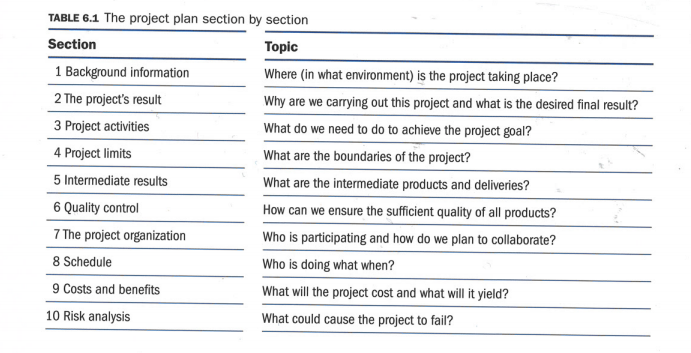
\includegraphics[width=14cm]{table.png}
\caption{\centering Dividing the project plan into sections as outlined by Grit et. al. \cite{Grit}.}
\label{table}
\end{figure} 
A brief summary of these sections are provided below.\\

\hl{Please note that you are expected to remove the guidelines provided in this template from the  Project Plan you submit, i.e. Incorporate your original work into this template and remove all the material presented as guidelines here. } %Remove this chapter
\chapter{Introduction $\&$ Background } Briefly introduce the project and provide some background information. Here you can include a short description of the layout of your project plan.



\chapter{Project Results }
\section{Physical objective}
The aim is to construct a loudspeaker system with a flat response due to the accuracy and quality of the filters, the amplifier, and the power supply.\\
We should be able to plug the speaker in and have music come out of it. The music should be split between 3 speakers: high frequencies come out of the tweeter, middle frequencies come out of the mid-speaker, and low frequencies from the woofer.\\
We should also be able to have an additional active filter for the bass level. 


\begin{itemize}
    \item Power supply: The power supply sub-group needs to create a circuit that brings down the input voltage of 230 volts to an average of 19 volts. Afterward, the AC input has to be transformed into a stable DC output. 
    \item Power amplifier: The power amplifier group have to filter out the bandwidth for the high/mid/low pass filters. Therefore the values of the capacitors and resistors must be chosen carefully to get the right bandwidth
    \item High/mid/low pass filters; The high/mid/low pass filters sub-groups need to filter out their specific frequencies. The filtered frequencies of the high, mid, and low pass filters should line up perfectly next to each other in order to prevent gaps or overlapping. 
\end{itemize}

    
    


\section{Learning objectives}
Besides creating a working sound system, the goal is to master certain learning objectives of the EPO project. After completion of the project, we will be able to apply the theoretical concepts of the first semester in practice.\\
Next, we have to achieve the basics of working in an engineering project group. the basics consist of planning, creating well-organized meetings, writing project plans, having the ability to give presentations, and writing engineering reports.\\
At last, we will achieve academic skills on a level that is expected of the university. for example being able to address specific problems, analyze data sheets and manuals, and critically assess and cit ate information.

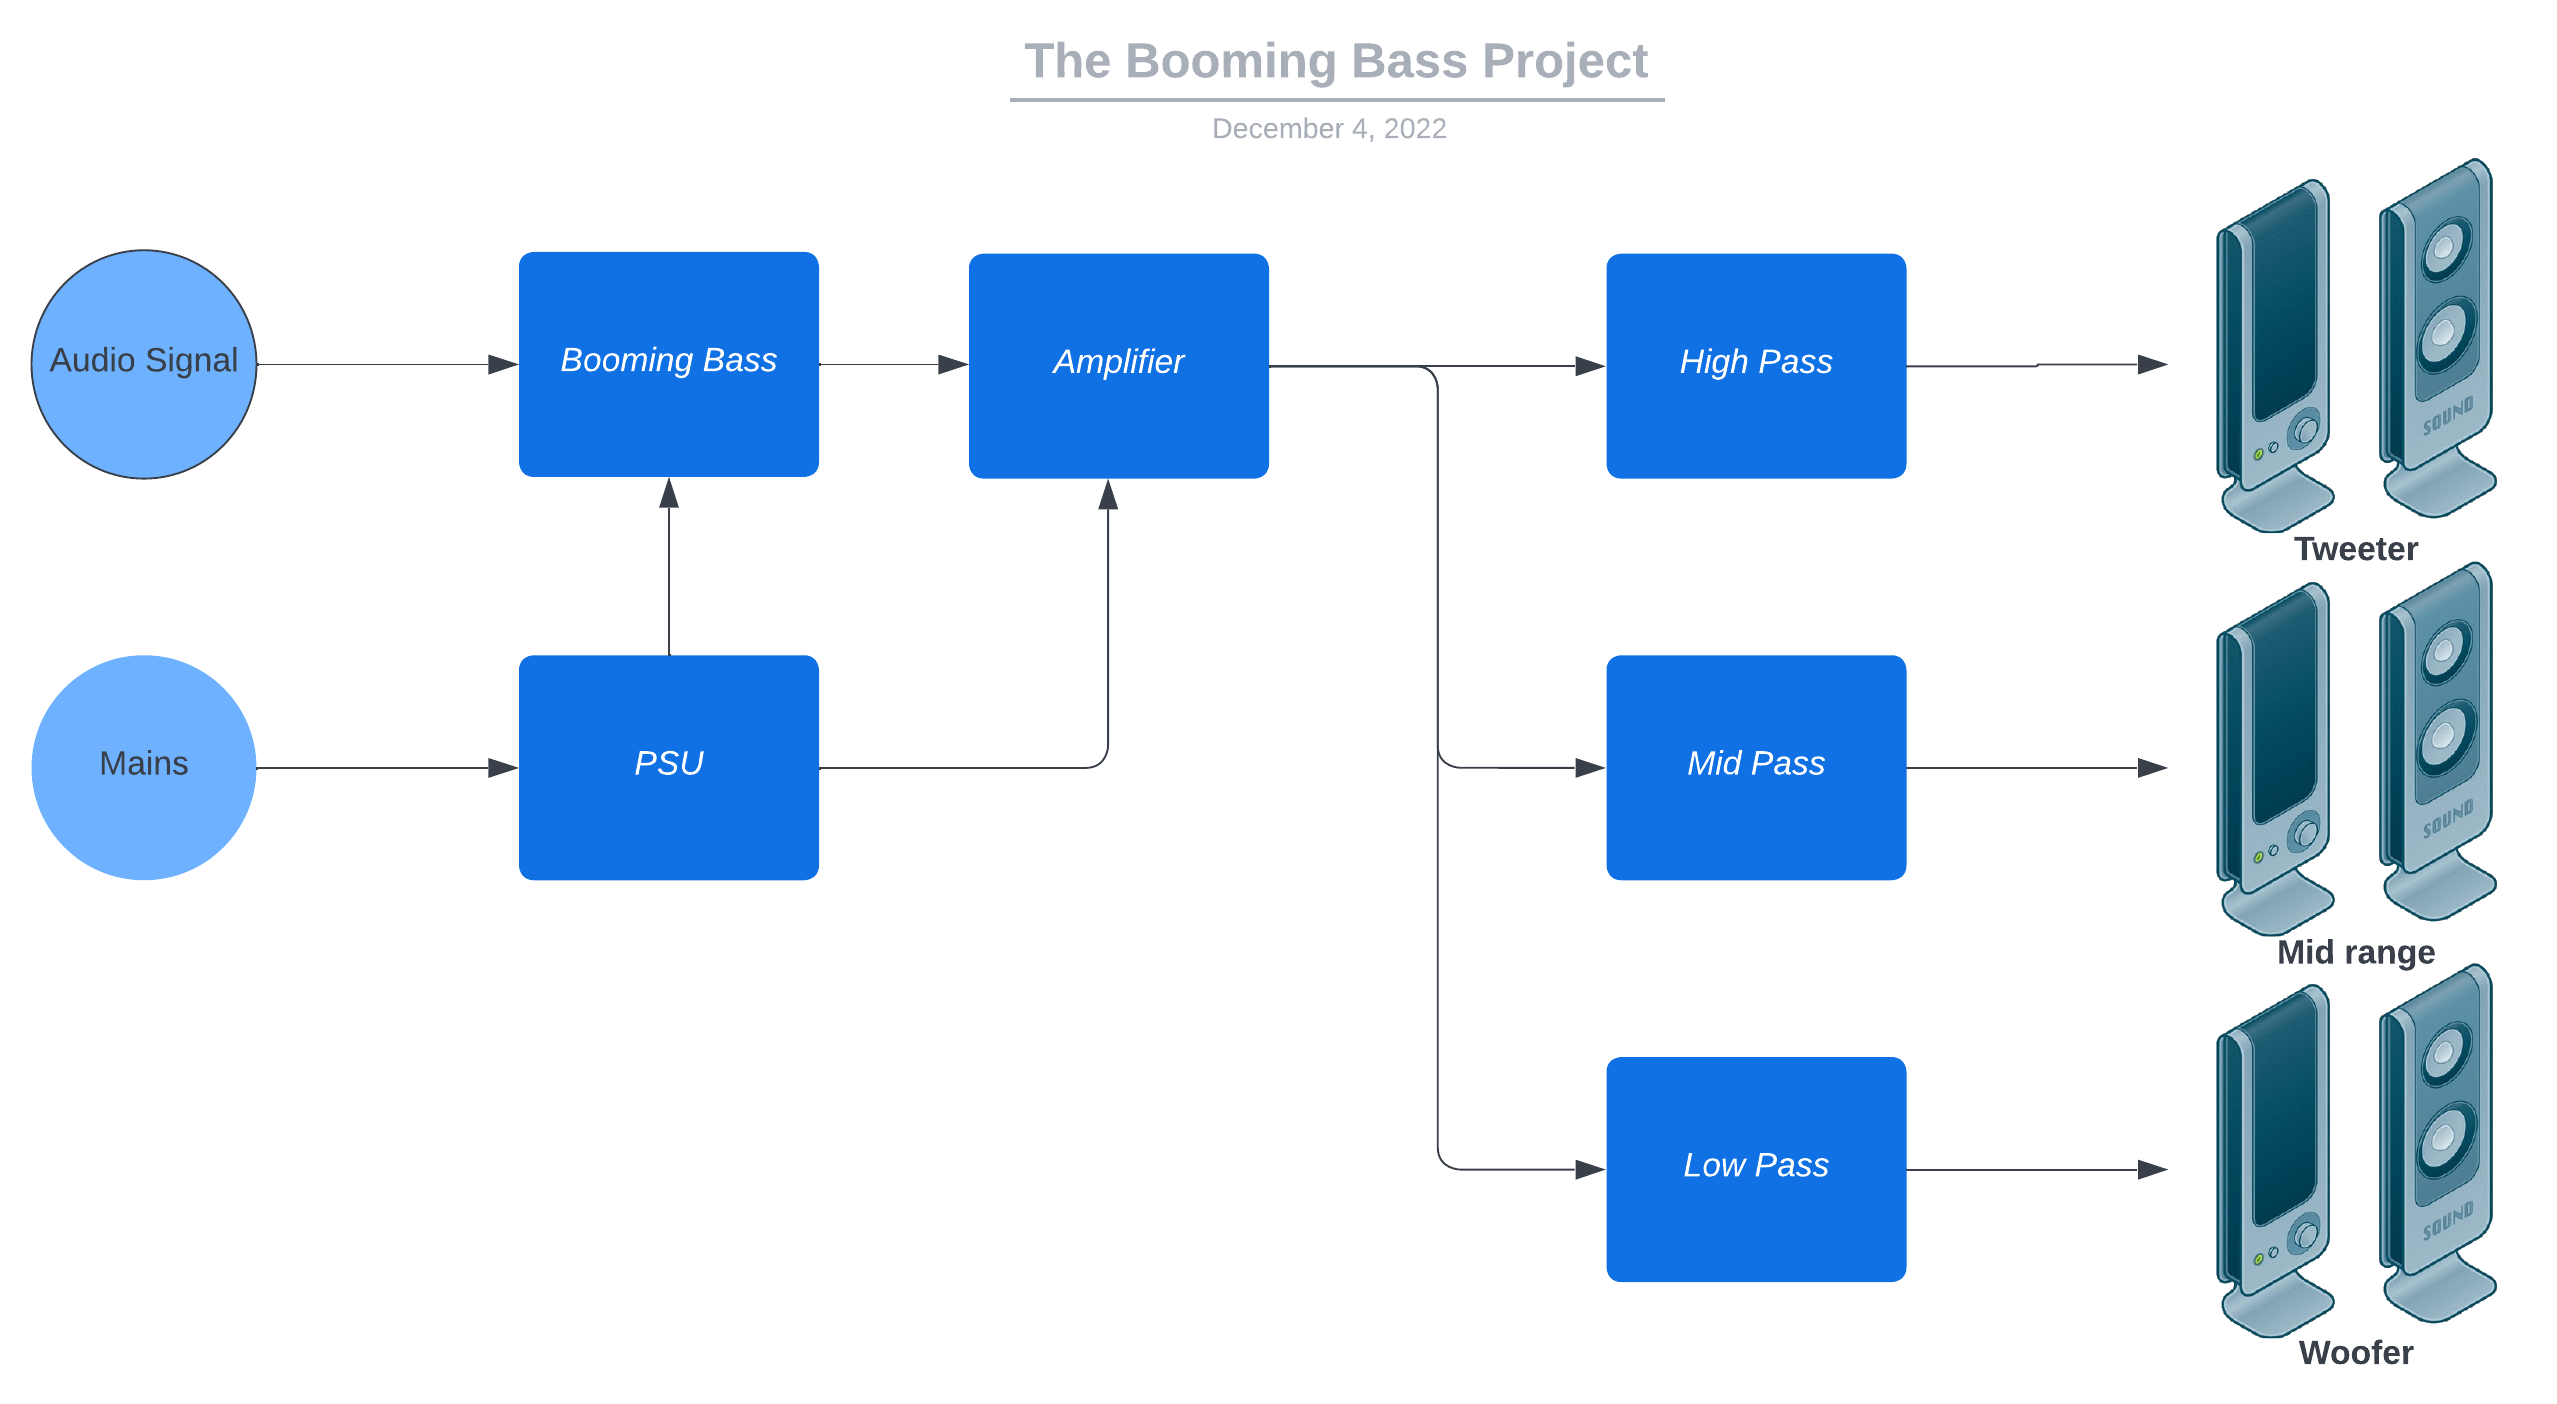
\includegraphics[scale=0.72]{Flowchart_1.png}










\chapter{Project activities}
In order to achieve the project's results, the group must divide the tasks well and communicate with each other clearly. In other words, work distribution has to be fair and meetings must be held regularly. A detailed description of the workload distribution with a timeline will be found in the next chapter.\\
\\
Regarding communication and file management, the group will use a shared Google Drive and WhatsApp. Each subgroup will upload each week's measurements, files, and calculations in the Drive.
In this chapter, we will briefly talk about what each group member will be doing and the roles of the meetings of the team. To finish the chapter, we will talk about the project limits.

\section{Task distribution}
As mentioned, efficient task distribution is key in order for the project to end well. Below you will find the subgroups of our project. Furthermore, in the appendix, you can find a compact work breakdown structure (figure 7.1) of each of the subgroups.
\subsection{Task distribution of A1\textunderscore1} 
\begin{table}[h]
\centering
\setlength{\arrayrulewidth}{0.5mm}
\setlength{\tabcolsep}{19pt}
\renewcommand{\arraystretch}{1.5}
    \begin{tabular}{|c|c|}
    \hline
    Power Supply     &  Maximiliaan Sobry, Ruben Noort\\
    \hline
    Power Amplifier     &  Thijs van Esch, Kevin Pang   \\
    \hline
    Low pass filter & Jeroen van der Werf, Dani van den Akker\\
    \hline
    Mid filter & Thijs Prakken, Wilson Rong \\
    \hline
    High pass filter & Pieter Olyslaegers \\
    \hline
    \end{tabular}
    \captionsetup{justification=centering}
    \caption{Subgroups A1\textunderscore1}
    \label{tab:my_label}
\end{table}
\newpage
\clearpage
\subsection{Task distribution of A1\textunderscore2}

\begin{table}[h]
    \centering
    \setlength{\arrayrulewidth}{0.5mm}
    \setlength{\tabcolsep}{19pt}
    \renewcommand{\arraystretch}{1.5}
    \begin{tabular}{|c|c|}
    \hline
    Power Supply     &  Adam Amnouh, Eliskan Karayi\v git\\
    \hline
    Power Amplifier     & \hspace{50pt}Wiktor Tomanek \hspace{50pt}   \\
    \hline
    Low pass filter & Darren van de Pol, Eojin Lim\\
    \hline
    Mid filter & Andy Zhang, Ishaan Sadal \\
    \hline
    High pass filter & Gijori Atmopawiro, Steven Bos \\
    \hline
    \end{tabular}
    \captionsetup{justification=centering}
    \caption{Subgroups A1\textunderscore2}
    \label{tab:my_label}
\end{table}


As mentioned, in the next chapter there will be a more detailed planning of each subgroup per week.


\section{Roles during meetings}
To have organized and useful meetings there must be roles during each meeting. Each group member will be the secretary and chairman for a week. Week 2.1 is not in the table, because that week was an introduction to this project, so no meetings were held.\\
\\
The chairman will lead and initiate meetings. On top of that, he will make sure that each subgroup is on track and that everyone is doing his job accordingly. The chairman is also the person to solve conflicts if they occur.\\
\\
The secretary will keep track of all the files and be responsible for the minutes during each meeting. Also, he will note all the progress, meetings and activities conducted by the group during that week. This way there is a clear overview of what has been done during the quarter and the progress made.
\newline

\begin{table}[!h]
\centering
\setlength{\arrayrulewidth}{0.5mm}
\setlength{\tabcolsep}{19pt}
\renewcommand{\arraystretch}{1.5}
    \begin{tabular}{|c|c|c|}
         \hline
         \makecell[l]{Week} & Chair & Secretary\\
         \hline
         2.2 & Dani & Wilson\\
         \hline
         2.3 & Wilson & Pieter\\
         \hline
         2.4 & Pieter & Jeroen\\
         \hline
         2.5 & Jeroen & Kevin\\
         \hline
         2.6 & Kevin & Maximiliaan\\
         \hline
         2.7 & Maximiliaan & Ruben\\
         \hline
         2.8 & Ruben & Thijs P.\\
         \hline
         2.9 & Thijs P. & Thijs v. E.\\
         \hline

    \end{tabular}
    \captionsetup{justification=centering}
    \caption{Roles during meetings A1\textunderscore1}
    \label{tab:Roles during meetings A1\textunderscore1}
\end{table}

\begin{table}[h]
\centering
\setlength{\arrayrulewidth}{0.5mm}
\setlength{\tabcolsep}{19pt}
\renewcommand{\arraystretch}{1.5}
    \begin{tabular}{|c|c|c|}
         \hline
         \makecell[l]{Week} & Chair & Secretary\\
         \hline
         2.2 & \hspace{10pt} Wiktor \hspace{10pt} & Mati\\
         \hline
         2.3 & Steven & \hspace{12pt} Gijori \hspace{12pt} \\
         \hline
         2.4 & Gijori & Ishaan\\
         \hline
         2.5 &  Ishaan & Andy\\
         \hline
         2.6 &  Andy & Darren\\
         \hline
         2.7 &  Darren & Eojin\\
         \hline
         2.8 &  Eojin & Eliskan\\
         \hline
         2.9.1 &  Eliskan & Adam\\
         \hline
         2.9.2 & Adam & Wiktor\\
         \hline

    \end{tabular}
    \captionsetup{justification=centering}
    \caption{Roles during meetings A1\textunderscore2}
    \label{tab:Roles during meetings A1\textunderscore2}
\end{table}

\newpage
\section{Project limits}

Every project has its limits, and this one is no exception. Some of these limits are the physical quality of the speaker, time limit, our ability to work together, the requirement of a passive circuit, our limited knowledge about speakers, no beforehand experience, circuitry etc. 


\subsection{Physical quality of the speaker}
This one is quite easy to explain. We have a limited amount of money so the components (capacitors, inductors, resistors etc.) will not be of top-notch quality, which means the physical quality of the speaker we are building will have some limitations. Nevertheless, we can maximize the quality of our speaker system by implementing our knowledge about electrical engineering as best as possible.

\subsection{Time limit}
Time is also a factor when we are talking about the limits of our system. The more time we have the better we can tweak, troubleshoot and solve problems. This means that we have to manage our time very well in order to deliver the maximum quality speaker, keeping in mind that we have limited time.

\subsection{Teamwork}
In order for us to complete this project we have to work as a team. Though, this is also a factor when it comes to our limitations. The quality of our project is somewhat limited by our ability to work together. This implicitly means that we have to set boundaries and communicate with each other as well as possible.

\subsection{Passive circuit}
For this project, the usage of a passive circuit for sound filters is mandatory. Also, each group is limited to the usage of 2 capacitors and 2 inductors. This results in less freedom for the group to choose their values for the capacitance and inductance, which subsequently limits the cutoff frequencies the group wants to choose for their filters. Therefore the group may not be able to make the optimal sound system, which is caused by a lack of sufficient capacitors and inductors.

\subsection{Limited knowledge}
The knowledge of the group is also limited. This will lead to the limited quality of the speaker system. There is still a lot to learn from the group members and this project is one way to do that. The members will also learn new things during the project to be able to complete the project, but not every member of the group may learn it on time, resulting in a delay caused by a group member(s).

\subsection{Experience}
Not every one of the group has experience with working in a large group on a project and for some of us, it is also the first time that we were assigned to do a project where they have to design and make a product. So there might be a difference in experience among the members of the group, which can possibly cause conflicts and delays.\\

Surely, there are more project limits, but these are the most important. It is therefore crucial to minimize the negative effects of these limits on our project whenever we can. 
\chapter{Organization $\&$ Schedule  } Make the distribution of workload among group members clear. Create a schedule which gives an overview of activities in relation to time (e.g., duration of each activity, start date, deadlines, etc). Based on these, carefully set your own timeline. Also think about the activities that (critically) influence the project and for which no explicit deadline is given in the manual.

For a group to work as efficiently as possible, there has to be a concrete plan to work toward the end goal. For this project, we have to work in four subgroups with each its own tasks. In this chapter, we will discuss what and when each group has to complete in order to fulfill the requirements for this project.\\

\section{Plan}
In table Schedule are all of the tasks described to whom or what subgroup has to do within a certain amount of time, which can deviate, from the corresponding deadline.

\section{Schedule}
In the table the letters E, S, C, SC and V stand for Everyone, Sensors, C-code, Serial communication and VHDL respectively.\\
\begin{table}[h]
\centering
    \begin{tabular}{| c | c | c |}
        \hline
        \textbf{Week} & \textbf{Subgroup} & \textbf{Task} \\
        \hline
        1 & E & \makecell[c]{Task distribution, reading the manual and\\ starting the project plan.}\\
        \hline
        1 & S & Sketching a general design of the mine sensor sub-circuit.\\
        \hline
        2 & S & \makecell[c]{Finishing the design, simulating and assembling\\ the analog board.}\\
        \hline
         3 & S & \makecell[c]{Writing the VHDL code for the frequency counter\\ and distance approximator.}\\
        \hline
        1 & V & \makecell[c]{Study manual and determine tasks\\ that need to be done for the VHDL (FSM) part of the project.}\\
        \hline
        1 & SC & \makecell[c]{Make tutorials in the manual and learn how to work with ZigBee.}\\
         \hline
        1 & C & \makecell[c]{Refresh C-coding and read through the manual.}\\
        \hline
        2 & C & \makecell[c]{Sketch a general design of the route planner and start coding it.}\\
        \hline
        3 & C & \makecell[c]{Finalize the route planner in C.}\\
        \hline
        2 & SC & \makecell[c]{Finish the tutorials and start the C code of the serial communication.}\\
        \hline
        2 & V & \makecell[c]{Start drawing FSD and writing the VHDL code and \\communicating with sensor and UART subgroup regarding their signals of the FSM.}\\
        \hline
        4 & C & \makecell[c]{Improve the C-code and remove any errors.}\\
        \hline
        5 & C & \makecell[c]{Test the improved C-code.}\\
        \hline
        3 & SC & \makecell[c]{Finalize the serial communication and eliminate possible errors.}\\
        \hline
        3 & V &  Continue writing the VHDL code for the FSM.\\
        \hline
        1 & 2 & 3\\
        \hline
        1 & 2 & 3\\
        \hline
        4 & V & Start finishing writing the VHDL code for the FSM.\\
        %% week 5: midterms
        \hline
        6 & V & Debugging the VHDL code if necessary and finishing the VHDL code.\\
        \hline
        1 & 2 & 3\\
        \hline
        1 & 2 & 3\\
        \hline
        7 & V & Debugging and finishing the VHDL code if necessary.\\
        \hline
        7 & E & Test with Roversim if possible.\\
        \hline
        8 & E & Testing and final symposium.\\
        \hline
        8 & E & Completing the final report.\\
        \hline
        9 & E & Preparing the oral presentation.\\
        \hline
        % week 8: final report deadline 15 June 22PM, note 15 june is also symposium.
    \end{tabular}
    \captionsetup{justification=centering}
    \caption{Schedule}
    \label{tab:Schedule}
\end{table}

\chapter{Risks Analysis } Make a brief risk analysis. Some examples on these risks are  too-little experience in the group for project-based approach, 
unavailability/underperformance of project members, lack of good 
collaboration and communication, etc.

\chapter{Conclusion} 
Conclude your report by providing a brief recap and discussion on your findings. 

\fi

\chapter{Introduction}

%requirements see manual
The introduction, a somewhat high-level, coarse and global description of the ’thing to be designed’, what function needs to be fulfilled, with a description of the overall characteristics.
2. The requirements, what are the quantifiable targets to be reached by the described module
\chapter{Mine Sensor}
%requirements manual

%%\textbf{3. The mine detector} \\
%%Motivate the choices between C and L detector. Describe at a circuit level the topology used and its operation. Do not forget to show the simulation of your circuit and compare it to the measurement results. Describe your extension for the detect mine. Describe at a circuit level the mine sensor topology used and its operation. Do not forget to show the simulation of your circuit. Describe your VHDL code extension for the detection of the mine. Describe at a circuit level the mine sensor topology used and its operation.


%mogelijke opmaak zie manual
\section{Introduction}

In EPO-2 the robot must be able to complete three different challenges. Two of these challenges are involved with obstacles in the robot's path, so called mines. The robot must be able to detect these mines in their path and avoid them by determining a different path that can be used to reach its destination. To detect these mines in the first place the robot must be equipped with a sensor which is able to detect these mines. In this chapter the design, testing, assembly and implementation of such sensor will be explained.

\section{The requirements}
The 'mines' on the field are made of metal disks.
Thus the first most important requirement is that the sensor must be able to sense iron objects.\\
In order to sense a metal object, another requirement is that a the circuit must be built with an LC oscillator.
%Idk more requirements

\newpage
\section{The followed design methodology}
\subsection{Design}





\subsection{Simulations}

The designed circuit should be first tested whenever the output of the circuit is indeed as expected, and whenever the frequency of the square wave output is indeed changing with a change of the inductance, which corresponds to the sensor sensing a metal object.

\begin{figure}[h]
    \centering
    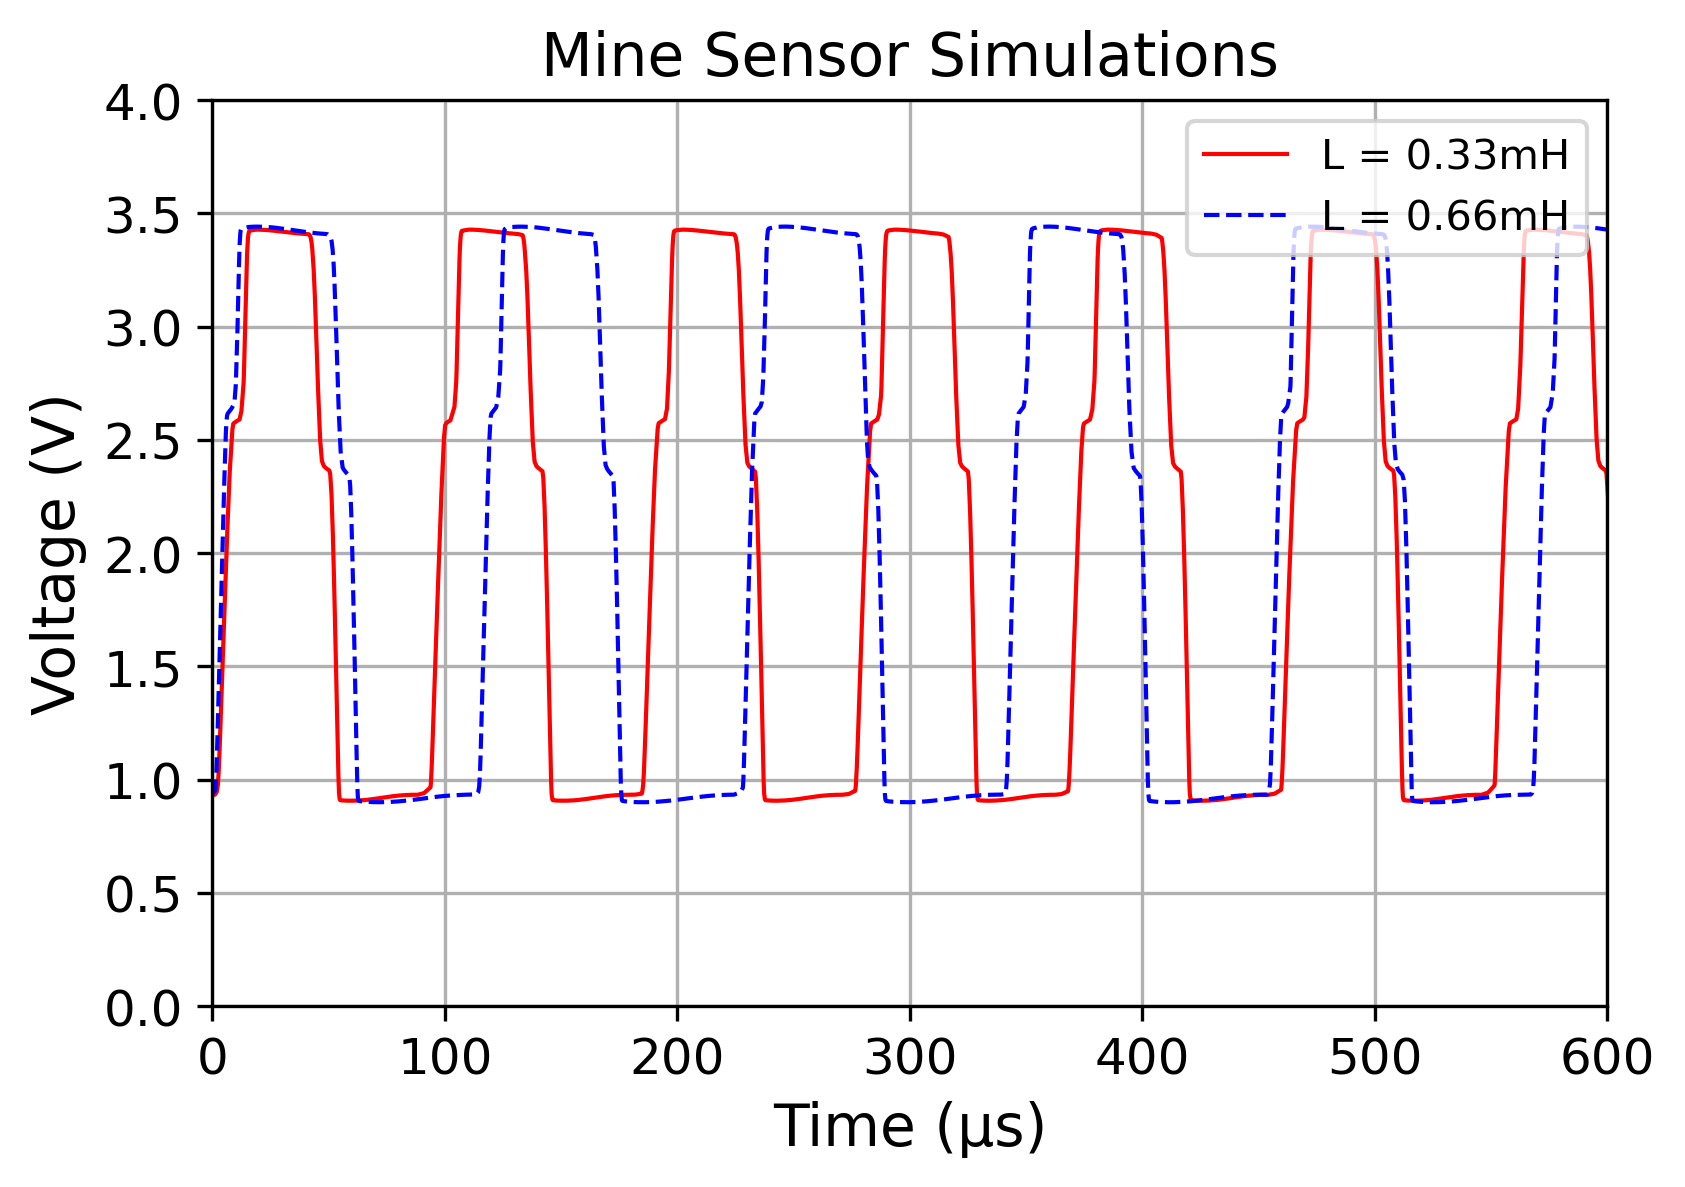
\includegraphics[scale = 0.7]{EPO 2 Images & Plots/Mine Sensor/666uH.png}
    \caption{Circuit Simulations}
    \label{fig:sim_sensor_neutral}
\end{figure}

Results of the simulations have shown the output of the circuit is indeed a square wave and the frequency of this square wave changes with an changing inductance value. In this case with an doubled inductance value from \(L=0.33mH\) to \(L = 0.66mH\) it is clearly shown in figure \ref{fig:sim_sensor_neutral} that the frequency of the square waves changes. An behaviour that should be expected. In the presence of the metal plate the inductance of the inductor increases giving a bigger period for the square wave. In reality the increase of inductance in presence of the 'mine' is around +10\%, this was measured using the XXX. %What was that decive called where you can measure all those components, inductance, capacitance and resistance.
In this simulation \(L=0.36mH\) is not given in the graph since the change in frequency is small and hardly noticeable in a graph. Nevertheless it doesn't matter that this value is not simulated since the main behaviour of; a changing period in presence of a changing inductance can also be simulated using \(L= 0.66mH\).\\
To sum up, the simulated output has a square wave function which period changes with a changing inductance. The simulated circuit works as expected.

\newpage
\section{Implementation}
\subsection{idk more things}
\\

\subsection{Code}
%Most likely this text has to be cut alot. To a more compact summary of the code.
After the sensor has been designed and simulated it will be built and integrated with the robot.
However, simply connecting the output of the sensor to the FPGA board is not yet enough. The output of this sensor still has to be processed to determine if a mine is detected or not.\\
With the use of some VHDL code the square wave output can be processed into determining whenever there is a mine detected or not.
As can be seen in the simulations, figure \ref{fig:sim_sensor_neutral}, the output of the sensor is a square wave functions. Which essentially has a high voltage and a low voltage, which the FPGA board reads as a '1' for high and '0' for low.\\
Since the '1' and '0' keeps its value for a few microseconds. We can count the amount of ones or zeros in 1 period. In presence of a metal mine, the inductance increases and thus also the period increases, which means the time the '1' and '0' holds in a period increases. Essentially if we know how many ones or zeros fit in one period without a mine. We can compare that with the amount of ones or zeros in a period with a mine. \\

Therefore the implemented code has a counter which in this case counts the amounts of zeros. In reality it doesn't really matter if the ones or zeros are counted, since the change in count due to a mine is important. The code is implemented using a FSM. The code has 4 stages, a reset stage, a counting stage, an compare stage, and a output stage. In communication with the other EPO-2 groups the output stage, the stage, which sends a '0' or '1' as output signaling that a mine had been detected, keeps on being on this stage for 10 milliseconds %%idk exact value anymore
so besides the FSM there is also a time counter which sends a '1' to the FSM when it is in the output stage and 10 milliseconds has passed. Which results the FSM to go back into its first stage, essentially resetting itself to start counting and detecting mines again. In the compare state the amount of zeros counted in one period gets compared to a set threshold. If it exceeds the threshold an '1' as output gets given in the output stage to the rest of the system, signaling a mine has been detected. The threshold for the code will be determined in the testing phase.

In Appendix XXX a visual FSD can be found and in Appendix XXX the code is given.

\subsection{Physical Placement Sensor}


\newpage
\section{The testing phase}
\subsection{Physical circuit testing}
After assembling the sensor circuit, it first will be tested whenever the circuit output also gives a square wave output as seen in the simulations.

Using a probe connected to the output, the output gets measured.

\begin{figure}[h]
    \centering
    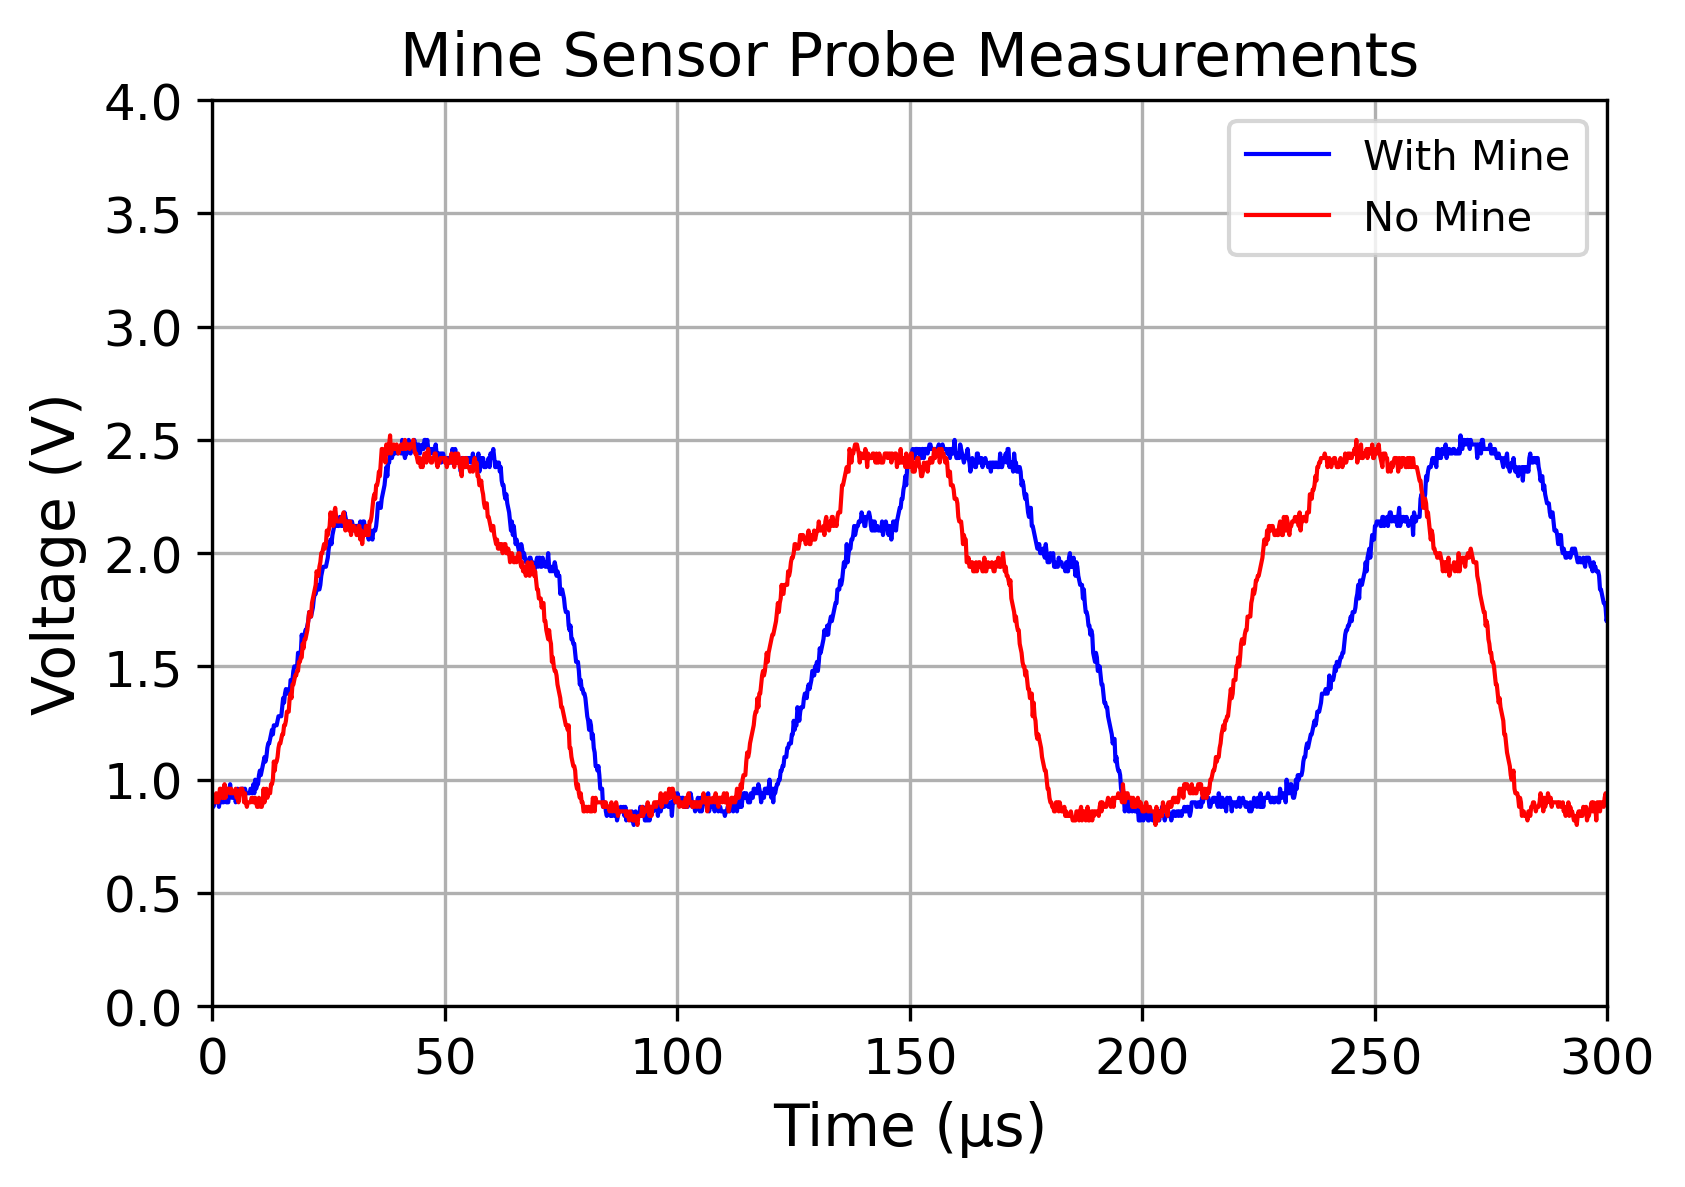
\includegraphics[scale = 0.7]{EPO 2 Images & Plots/Mine Sensor/V3_Total.png}
    \caption{Circuit Probe Measurements}
    \label{fig:meas_sensor_neutral}
\end{figure}

As seen in figure \ref{fig:meas_sensor_neutral} the output is mostly a square wave function. The FPGA board considers voltages above 1.2V as a '1'. So the two 'steps' are seen as a '1'. Essentially when looking carefully at the measurements, the amount of time that the signal is a '1' is longer than it is '0' in a period. This is not problematic since the change in the period under influence of a mine is important. So the shape of the 'square' wave signal is fine.\\
In figure \ref{fig:meas_sensor_neutral} the square wave is plotted with and without a mine. The graph shows a clear change in frequency and with a mine the period is bigger. Which is expected from the simulations. From this it can be concluded the sensor sufficiently senses the presence of a mine.\\
After testing the built circuit works as intended, the next step is to determine how many times '0' gets counted in 1 period. With this information a treshhold value can be set in the VHDL code.\\
The FPGA boards runs on a 50Mhz clock which has a 20 microseconds period. It must be determined how many of these 20 microseconds periods fit into the '0' state of the output square wave signal of 1 period. The time the signal is below the 1.2V could be measured with a oscilloscope. However the decision is made not to do this and instead to use the FPGA board directly to count the '0' state of the square wave. This is so that in the unlikely event that the circuit may behave a bit different on the FPGA board, the counted value is exactly is the actual value the FPGA board counts.
%%bla bla not yet finished.


\newpage
\subsection{Sensor FPGA board implementation testing}
A simple VHDL code which counts how many periods of 20 microseconds fit into the low state of the square wave for 1 period was written, with a bit vector as output. This output was displayed on the FPGA board using the leds. This gave 2112 counts without a mine and 2400 counts with a mine.
After further testing and testing with the actual VHDL sensor code with the different values as threshold. A final threshold value of 2350 counts was chosen.\\

After a threshold was chosen the sensor with VHDL code can be tested. After the VHDL Code was implemented on the FPGA board. Two states, the counting stage and the compare stated where checked if they work as intended. By designating a led to each state, a probe was connected to the led to see the states on the oscilloscope.

\begin{figure}[!h]
    \begin{minipage}{0.5\textwidth}
     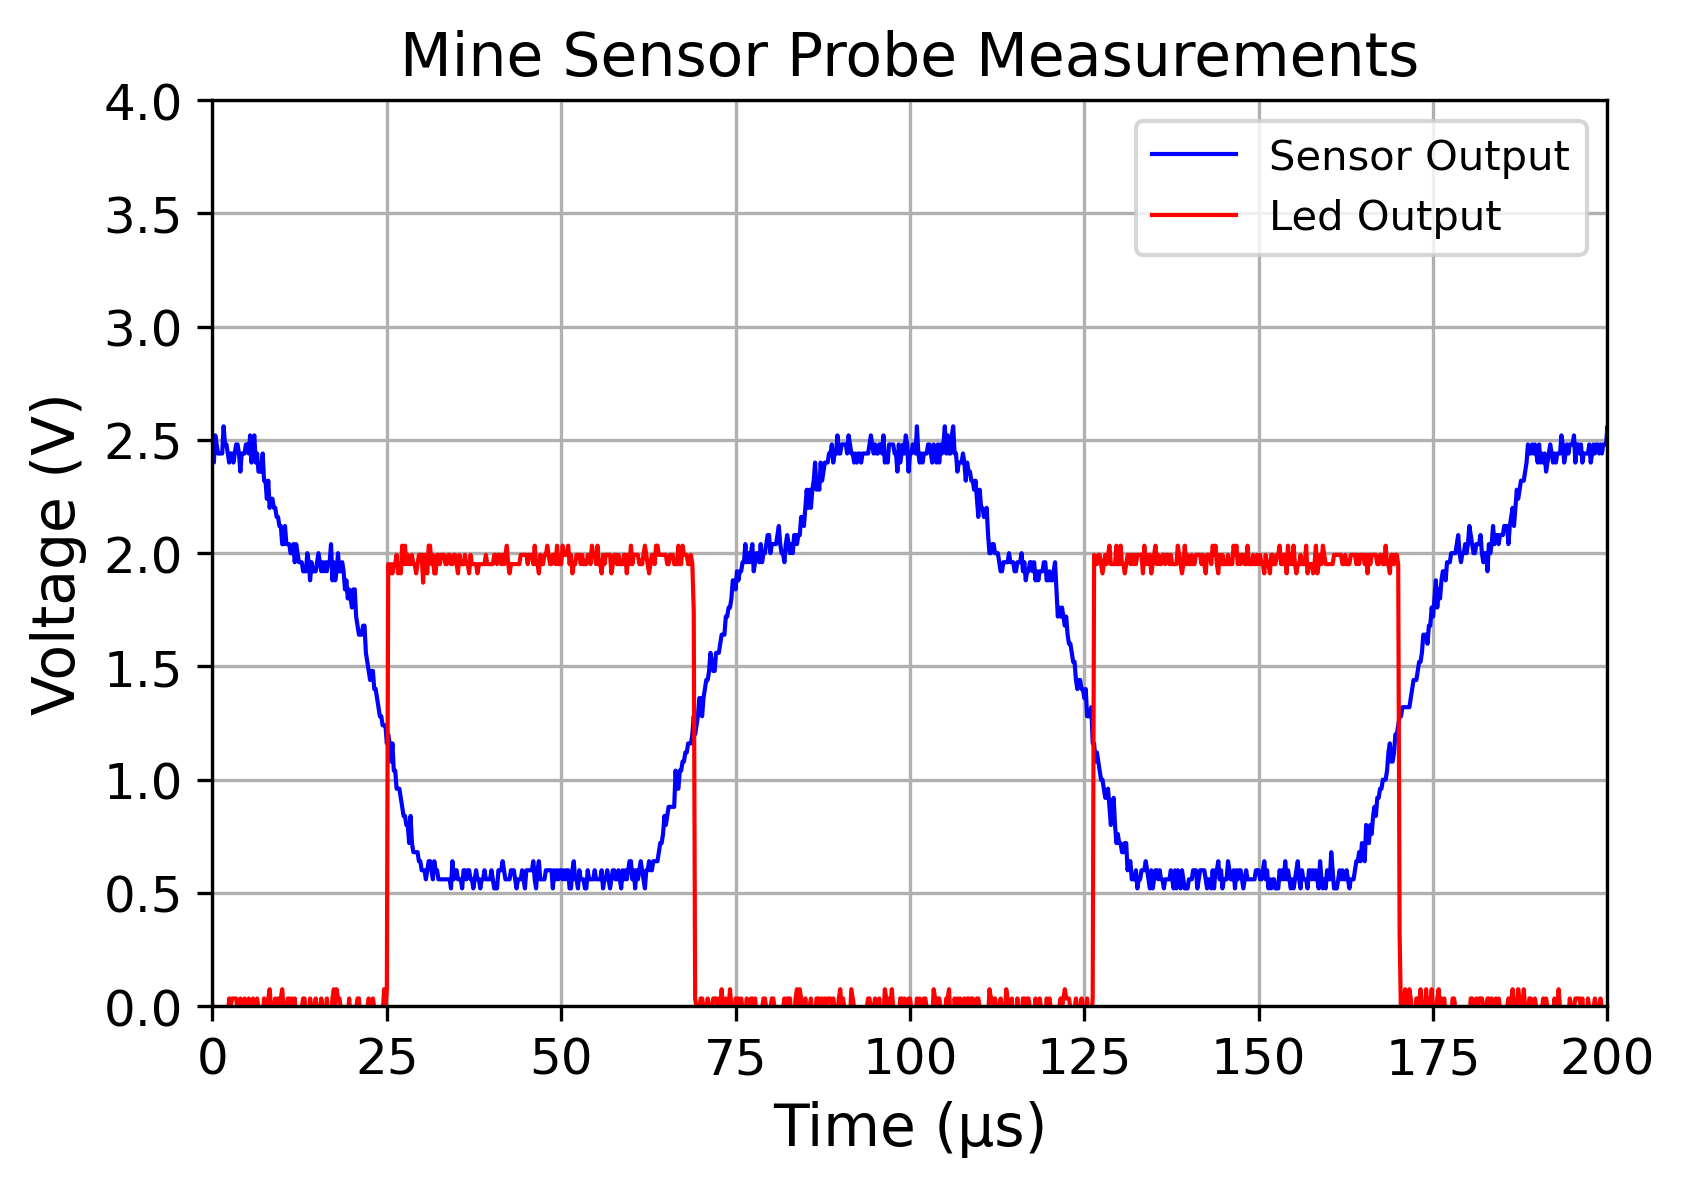
\includegraphics[width=\linewidth]{EPO 2 Images & Plots/Mine Sensor/V3_Count_Stage_No_Mine.png}
     \caption{Count state}
     \label{fig:meas_count}
    \end{minipage}
    \hfill
    \begin{minipage}{0.5\textwidth}
      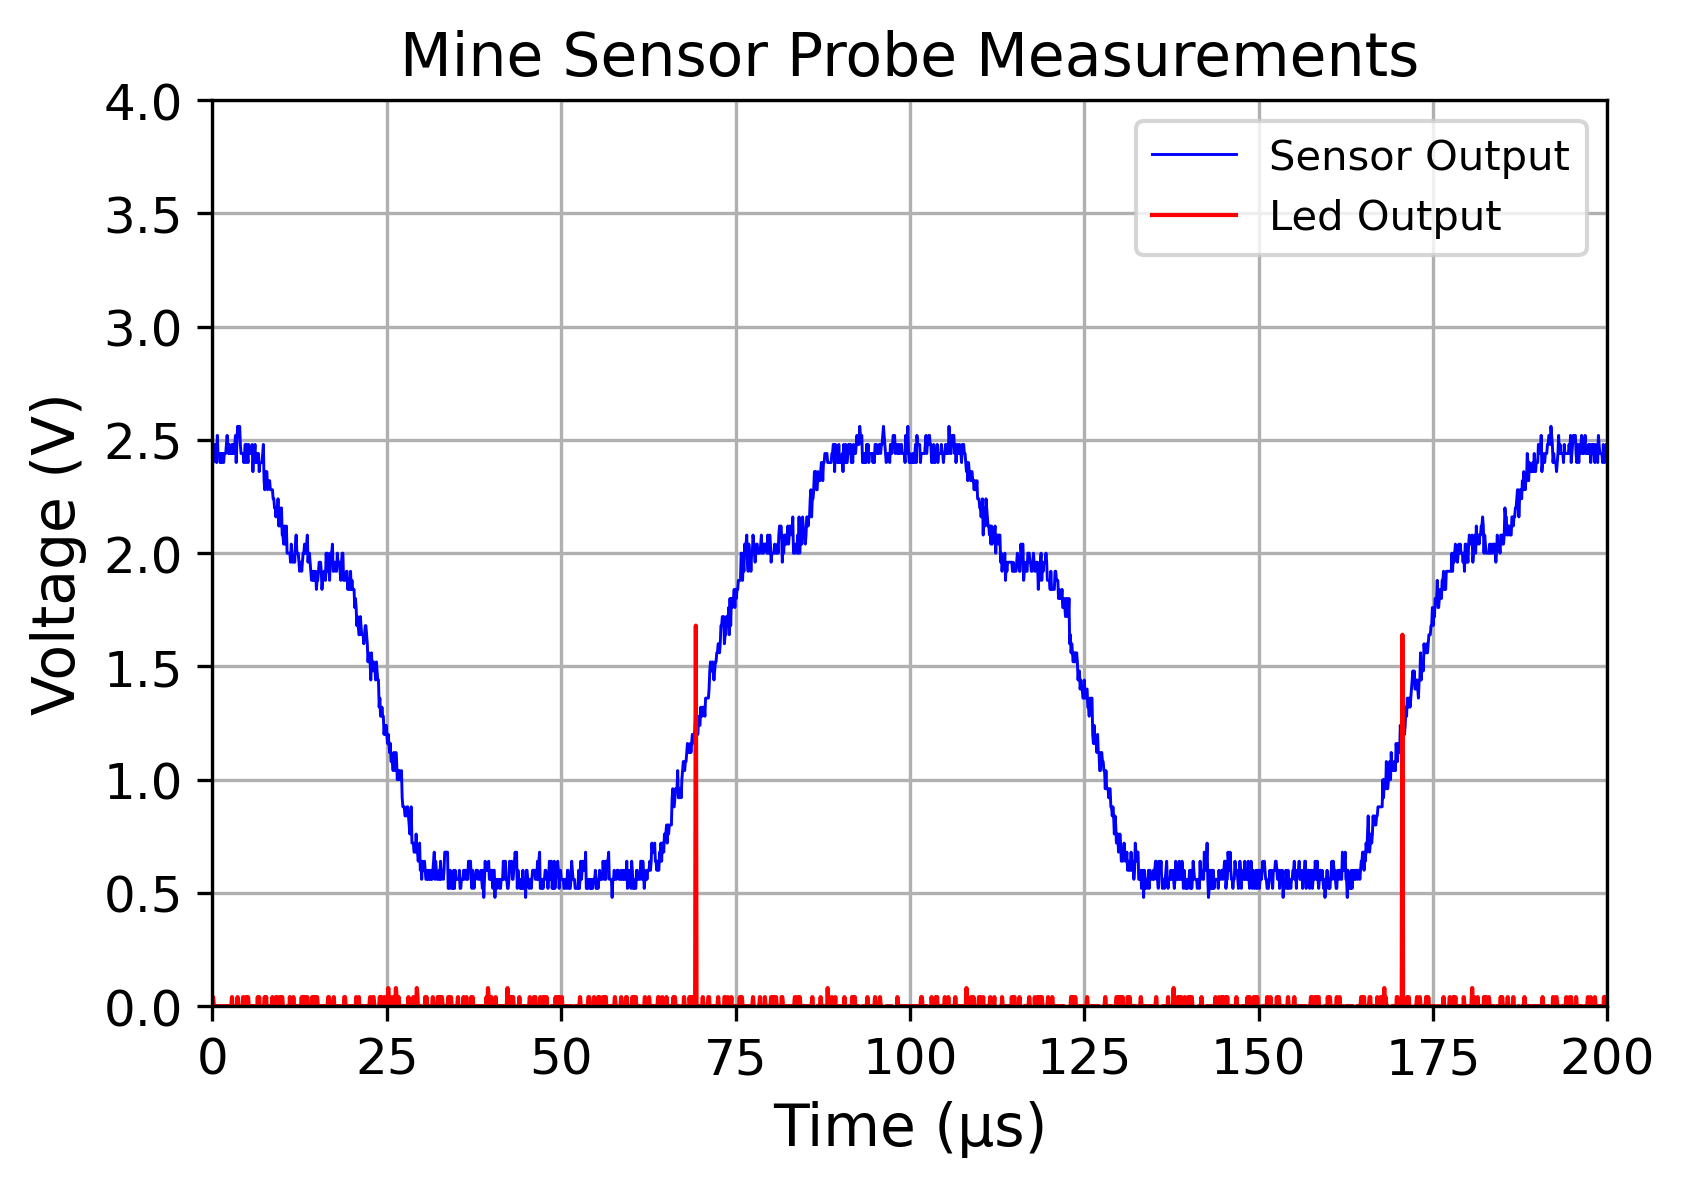
\includegraphics[width=\linewidth]{EPO 2 Images & Plots/Mine Sensor/V3_Compare_State_No_Mine.png}
      \caption{Compare state}
      \label{fig:meas_compare}
    \end{minipage}
\end{figure}

As can be seen in figures \ref{fig:meas_count} and \ref{fig:meas_compare} the counting state can be seen when the square wave signal is '0' and the compare state can be seen at the end of the '0' signal when the square wave jumps to a higher voltage. This shows us the VHDL Code is indeed counting when the square wave signal is low and after counting immediately goes to the compare state. Out of visual observations where the output in the output state is assigned to a LED. It could be seen that the LED lights up when an metal object is placed below it and stays off when there is nothing below the sensor. From these observations and measurements it can be said confidentially that the sensor and the code works as intended.


\chapter{C}

%requirements manual
\textbf{The route planner on the PC (only in final report)} \\
Describe how the route planner on the PC works, detail the algorithms you have implemented to complete the various challenges (i.e., A, B and possibly C) (note if the section becomes too lengthy can be added in the appendix).

%mogelijke opmaak zie manual
\section{Introduction}

\section{The requirements}

\section{The followed design methodology}

\section{Implementation}

\section{The testing phase}

\chapter{VHDL}
%%TA zei dat het ook mogelijk is om linefollower toe te voegen in epo2, bijv een beschrijving van hoe je de linefollower hebt aangepakt en hoe je hebt getest en geverifieerd dmv testbench.

\section{1. The line follower}
Remember the process you did to understand the operation: creating a time base, testing the effect of the PWM, use the inputs of the light sensitive sensors and defining an FSM to control the process.
Translate this process in a concise way, avoiding repetition to the manual content, in a chapter describing: Requirements, Design, Implementation and Testing phase.

\textbf{Line follower}
the frequency of the clock is 50MHZ, which means that the tril

\textbf{Light-sensitive sensors}
%Chantal: use the inputs of the light-sensitive sensors manual LF p6
Light-sensitive sensors need to be used to detect what the robot observes. The light-sensitive sensors measure the reflection from the ground. Their circuit can set the output to '0' or '1', respectively black and white. With the sensor output a VHDL code can be written so that the robot can detect what they need to do based on what he observes. For example when the robot observes '110', white white black, with the light-sensitive sensors and he got the task to go forward. Then the robot will correct himself and turn gently left till he observes '010', white black white.\\

\textbf{Time Base}
%%Chantal: PWM and the 20-bit vector for counter LF manual p8 and creating a time base p38
A time base needs to be created for the robot to measure the time within a period of the pulse width module (PWM) signal. The PWM signals control the server motors and is therefore used for the motion of the robot. To get the right PWM signals a counter consisting of 20 bits needs to be used. Since the general clock has a counter of MHz and the PWM sends a pulse every 20 milliseconds. 
\textbf{Inputbuffer}

\textbf{Controller}


\textbf{Motor controll}

\\
\\


\textbf{Changes made for a mine detector robot}

\textbf{Adapted controller from the line follower}
%Chantal: testing the effect of the PWM  (maybe bij testing) manual LF p7
The robot needs to turn 90 degrees when they get the order to turn left or right. To get the closest turn to 90 degrees a test code, based on the line follower code, has been written and executed. With trial and error a PWM of .... milliseconds has been chosen. \\

For the correct movements of the robot, the final state machine of the line follower needs to be expanded. This final state diagram only implements what the robot needs to execute when receiving a code from the PC. Therefore, the C-code will become the brain of the system and VHDL will solely follow its order. The communication between the C-code and the VHDL is described in chapter \ref{chapter_communication}. Only when the robot is riding forward, meaning that the robot is in the forward\textunderscore{state}, the robot will follow and correct the line.\\

The following final state machine has been implemented: \\
%% figuur FSD

The VHDL code for the final state machine in figure %verwijzing naar figuur%
has been described in Appendix \ref{appendix_linefollower}
\\

%mogelijke opmaak zie manual
\section{Introduction}
In this project, the robot must be able to drive forward, turn left and right. This is achievable by sending the correct PWM signals to the robot. Therefore, a Final State Diagram with accurate output signals must be designed.

\section{The requirements}

\section{Design}

\section{Implementation}

%%Eojin
In the given manual \cite{EPO2_manual} there are two (optional) example approaches. The first approach is expanding the FSM of the line follower (A project that had to be completed in pairs before EPO 2 began). This has its pro's and cons: 
\\


Het idee:
1. FSD tekenen met de requirements
2. VHDL code schrijven aan de FSD
3. Debuggen zo mogelijk
4. Samenvoegen met C en dan verwijzing naar communication.
5. Testing the PWM, hoe veel moet hij naar links en naar rechts.

\section{Testing phase}

There have been some trials and errors in the VHDL code. %uitleg wat er fout ging
\chapter{Communication}
\label{chapter_communication}

%% Zie github
%requirements see manual
\textbf{The wireless communication module} 
 Give a top level view of the operation of the wireless link. Describe the protocol and the error recovery measures (in case implemented). Describe eventual test-benches that were used and the testing procedure with the robot to validate the proper operation of the link.


\textbf{The robot controller on the FPGA}
Describe the way the controller navigates the robot through the maze using the inputs from the sensors (mine and light sensitive sensor) and the information received from the route planner. Also how the data are transmitted between the PC and robot. Be accurate in the usage of fine state diagrams. Report the test protocols you have used to validate the proper functioning of the robot.

%mogelijke opmaak zie manual
\section{Introduction}

In order to ensure that the robot can receive the right order, there must be communication between the C and the VHDL-code. The C-code can be seen as the brain and the VHDL-code as the body of our system.


\section{The requirements}

\section{The followed design methodology}
%%Misschien hier nog een short introtje erbij ofz
%%Chantal: vgm hoort het stuk van Thijs op Github bij dit stukje maar ik weet dat niet zeker

\subsection{Communication between robot and controller}
In this EPO-2 project, it is decided that the programming language C is the brain and VHDL the body of our system. This section contains the technical description of the communication between the robot (controlled by the FSM created by VHDL team) and the controller (an application in C programming language running on a desktop written by C team).

\textbf{\subsubsection{Send data or receive data?}}
This section describes when to read or receive data from the perspective of the robot. This means that data sent by the
robot to the desktop will be referred as 'outgoing data' and data sent by the controller to the robot will be 
referred as 'incoming data'.


The following flowchart described when both the robot and the control should send byte and when they should expect to
receive a byte.

%%Foto Images/commination.png (Thijs, zie Github)

Both the controller and robot have to send one byte and receive one byte per cycle. The controller is the entity that
sends the first byte. For every byte sent by the controller to the robot, the robot should send a byte back to the controller, before the robot executes the byte from the controller. This way, the controller knows that the byte is received well by the robot. By doing this, the chances of miscommunication between controller and robot decreases enormously, which will lead to a proper end product.

\textbf{\subsubsection{Incoming data}}
This section describes the format of the incoming data byte. This byte is sent by the controller to the robot.

Only the three least significant bits (bits 2, 1 and 0) contain data. The remaining five bits always have the value 
'0'. The three bits that actually contain data represent the opcode of the operation that the robot should execute.
All possible combinations of these bits with the corresponding operations are listed in the table below.

\begin{longtable}[c]{| c | c | c |}
        \hline
        \textbf{Operation} & \textbf{Opcode} & \textbf{Meaning} \\
        \hline
        `ROBOT\textunderscore{NOOP}` & 000 & The robot should keep doing what it was already doing.\\
        \hline
        `ROBOT\textunderscore{LEFT}` & 001 & The robot should start rotating to the left.\\
        \hline
        `ROBOT\textunderscore{RIGHT}` & 010 & The robot should start moving to the right.\\
        \hline
        `ROBOT\textunderscore{FORWARD}` & 011 & The robot should start moving forward.\\
        \hline
        `ROBOT\textunderscore{STOP}` & 100 & The robot should stop rotating or moving forward. It should come to a stop. \\
        \hline
        - & 101 & Illicit opcode.\\
        \hline
        - & 110 & Illicit opcode.\\
        \hline
        - & 111 & Illicit opcode.\\
        \hline
    \captionsetup{justification=centering}
    \caption{Combination of bits sent from controller to robot \label{bits_controller_to_robot}}\\
\end{longtable}

\textbf{\subsubsection{Operation priority}}
The robot may assume that after a `ROBOT\textunderscore{LEFT}`, `ROBOT\textunderscore{RIGHT}` or a `ROBOT\textunderscore{FORWARD}` has been sent, the next operation
that is not `ROBOT\textunderscore{NOOP}` will always be `ROBOT\textunderscore{STOP}`. 

In other words, the robot is assumed to always be in a state of not doing anything when 'ROBOT\textunderscore{LEFT}`, `ROBOT\textunderscore{RIGHT}` 
or `ROBOT\textunderscore{FORWARD}` is sent as operation.

\textbf{\subsubsection{Outgoing data}}
This section describes the format of the outgoing data byte. This is the byte that is sent by the robot to the
controller. This byte is to be sent exactly once after each time an incoming data byte is read.

Each bit in the outgoing data byte indicates a piece of data. The meaning of each bit is described in the table below.

\begin{longtable}[c]{| c | c | c |}
        \hline
        \textbf{Position of the bitvector} & \textbf{Name} & \textbf{The binary digit of the bitvector} \\
        \hline
        data\textunderscore{out}[7] & rotatingLeft & \makecell[c]{Should equal '1' if the robot is currently rotating to the left,\\ '0' otherwise..}\\
        \hline
        data\textunderscore{out}[6] & rotatingRight & \makecell[c]{Should equal '1' if the robot is currently rotating to the right,\\ '0' otherwise.}\\
        \hline
        data\textunderscore{out}[5] & isDriving & \makecell[c]{Should equal '1' if the robot is \\currently rotating or the robot is moving forward.}\\
        \hline
        data\textunderscore{out}[4] & sensorLeft & Should equal the value outputted by the left line sensor.\\
        \hline
        data\textunderscore{out}[3] & sensorMiddle & Should equal the value outputted by the middle line sensor. \\
        \hline
        data\textunderscore{out}[2] & sensorRight & Should equal the value outputted by the right line sensor. \\
        \hline
        data\textunderscore{out}[1] & mineDetected & \makecell[c]{Should equal '1' if the robot is currently detecting a mine,\\ '0' otherwise.}\\
        \hline
        data\textunderscore{out}[0] & readBit & \makecell[c]{Should equal '1' if the data contained \\within the rest of the byte is to be read.}\\
        \hline
    \captionsetup{justification=centering}
    \caption{Feature represented by the position of the data\textunderscore{out}-vector \label{scheme_data_out_vector}}\\
\end{longtable}

\textbf{\subsubsection{Sensor data}}
Bits 4, 3 and 2 contain the left, middle and right line sensor values, respectively. The controller interprets the
meaning of the values of these bits as follows.

If such a bit has value '0', the controller assumes that the corresponding sensor is currently detecting a line. If
such a bit has value '1', the controller assumes that no line is detected.

\textbf{\subsubsection{The readBit}}
The controller always desires to read the byte that was sent by the robot. When the readBit is 1, this means that the controller reads the byte sent by the robot. 

After the VHDL receives a signal from C-code, it will follow the order contained in the signal by going to the appropriate case. Following the same example, only the VHDL-code written in the case forward (described in the FSD) will be executed. After receiving the confirmation signal, the C-code will -- milliseconds in order that the VHDL code can execute the case which has been given by the signal. 
%% aantal ms moet nog worden gegeven door C

\section{Implementation}

\section{The testing phase}
After the C-code and VHDL-code was written, it was tested if the robot worked correctly. The biggest problem that was encountered was that not the right std\textunderscore{logic}\textunderscore{vector} was sent back to the controller.

To solve this problem, the FSD was changed to meet the requirements for better communication between controller and the robot. The changes involve ...



Also a few small problems were encountered as forgetting a new\textunderscore{state} in the VHDL-code.

\chapter{Conclusion}

%requirements manual
\textbf{Test results of the robot performance in the challenges} //
Approach and report on the test plan in a scientific way, be precise in the reporting of numerical data
(number of digits, accuracy, etc.)
\chapter{Notes}

08-05-2023

C group came with a suggestion to become the brain of our system and let VHDL solely follow its order. This will lead to two advantages: It is easier to perform the same task if the task is written in C than in VHDL and the FSM of VHDL decreases a lot, which leads to less work for the VHDL group. Needless to say, everyone agreed to implement this suggestion and more is explained in the chapter VHDL or C (must be decided yet) \newline


11-05-2023
The VHDL team forgot to add a mine-reset state in their FSM. After discussing with C and sensor group, it was decided that the sensor group will add a timer to their own written FSM, which ensures that the signal is 1 for 40ms when a mine is detected by the mine sensor. That signal is sent to the PC , which in turn will return a signal that contains the order to make a U-turn, to the VHDL.It is better that transmission of mine-detection is between C and sensors because C is much faster  than VHDL.

Looking back, the original FSM contained unnecessary states (the check states). By removing them, this will lead to less usage of states, which will make the robot faster. This is possible because the robot can read and write in the same state. It was not previously considered that the robot could execute motor commands and write to the Xbee simultanously. 



2023-05-15
Testing Communication: 
The robot stopped when C language had given a stop signal and a forward signal respectively during the communication between C language and VHDL.

-> missing newstate

sensorlmr worden niet goed assigned bij de stdlogicvector die naar de C-code wordt gestuurd
-> new fsd state met de hoop dat ie het doet

2023-06-01
De VHDL code switched te snel van state, het loopt niet 20 ms in de state. Hierdoor gaat hij te snel naar de volgende state en heeft hij niet genoeg tijd te lezen.

%% Use letters for the chapter numbers of the appendices.
\appendix
\chapter{Line Follower} 
\label{appendix_linefollower}
%zou fijn zijn als iemand hier een intro voor kan schrijven
%NOTE CONTROLLER EN ROBOT ZITTEN ER NIET IN, EN DE TESTBENCH ZITTEN ER NIET IN.

\section{Timebase}
\begin{lstlisting}[style=vhdlStyle]
library IEEE;
use IEEE.std_logic_1164.all;
use IEEE.numeric_std.all;

entity timebase is
	port (  clk             : in std_logic;
        	reset           : in std_logic;
        	count_out       : out std_logic_vector (19 downto 0)
 	) ;
 end entity timebase ;

 architecture behavioural of timebase is

 	signal count, new_count : unsigned (19 downto 0);

 begin
 	process ( clk )
 	begin
 		if ( clk'event and clk ='1' ) then
			if ( reset = '1' ) then
 				count <= ( others => '0');
 			else
 				count <= new_count;
 			end if;
 		end if;
 	end process;


 	process ( count )
 	begin

		new_count <= count + 1;

 	end process;

 	count_out <= std_logic_vector ( count );
 end architecture behavioural;
 \end{lstlisting}

\newpage
\section{Motorcontrol}
 \begin{lstlisting}[style=vhdlStyle]
 library IEEE;
use IEEE.std_logic_1164.all;
use IEEE.numeric_std.all;

-- Please add necessary libraries:

entity motorcontrol is
	port (	clk		: in	std_logic;
		reset		: in	std_logic;
		direction	: in	std_logic;
		count_in	: in	std_logic_vector (19 downto 0); 

		pwm		: out	std_logic
	);
end entity motorcontrol;

architecture behavioural of motorcontrol is
	
	type motorcontrol_state is (state0, state1, state2);

	signal state, new_state: motorcontrol_state;

begin 

    process (clk)
    begin
	if (rising_edge (clk)) then
		if (reset = '1') then
    		state <= state0;
		else
				state <= new_state;
		end if;
	end if;
    end process;


    process (direction, count_in, state)
    begin
	case state is

    	when state0 => pwm <= '0';
				new_state<=state1;
			
			when state1 => pwm <= '1';
				if (direction ='0' and unsigned(count_in) >= to_unsigned(50000, 20)) 
                                    then new_state <= state2;
					
				elsif (direction ='1' and unsigned(count_in) >= to_unsigned(100000, 20)) then
				    then new_state <= state2;

				else
					new_state <= state1;
				end if;


			when state2 => pwm <='0';
				new_state <= state2;

		end case;
	end process;
end architecture behavioural;
 \end{lstlisting}

\newpage
\section{Inputbuffer}
 \begin{lstlisting}[style=vhdlStyle]

 library IEEE;
use IEEE.std_logic_1164.all;
use IEEE.numeric_std.all;
-- Please add necessary libraries:


entity inputbuffer is
	port (	clk		: in	std_logic;

		sensor_l_in	: in	std_logic;
		sensor_m_in	: in	std_logic;
		sensor_r_in	: in	std_logic;

		sensor_l_out	: out	std_logic;
		sensor_m_out	: out	std_logic;
		sensor_r_out	: out	std_logic
	);
end entity inputbuffer;

architecture structural of inputbuffer is

component flipflop is 

	port(clk, sensor_l_in, sensor_m_in, sensor_r_in: in std_logic;  
                sensor_l_out, sensor_m_out, sensor_r_out: out std_logic);
end component;

signal s1, s2, s3: std_logic;

begin 

FF1: flipflop port map(	clk => clk, 

			sensor_l_in => sensor_l_in, 
			sensor_m_in => sensor_m_in,  
			sensor_r_in => sensor_r_in, 

			sensor_l_out => s1,
			sensor_m_out => s2,
			sensor_r_out => s3);

FF2: flipflop port map(	clk => clk, 

			sensor_l_in => s1,
			sensor_m_in => s2,
			sensor_r_in => s3,

			sensor_l_out => sensor_l_out,
			sensor_m_out => sensor_m_out,
			sensor_r_out => sensor_r_out);

end structural;
 \end{lstlisting}

\newpage
\section{3bit\textunderscore{flipflop}}
 \begin{lstlisting}[style=vhdlStyle]
 library IEEE;
use IEEE.std_logic_1164.all;
use IEEE.numeric_std.all;
-- Please add necessary libraries:


entity flipflop is
	port (	clk		: in	std_logic;

		sensor_l_in	: in	std_logic;
		sensor_m_in	: in	std_logic;
		sensor_r_in	: in	std_logic;

		sensor_l_out	: out	std_logic;
		sensor_m_out	: out	std_logic;
		sensor_r_out	: out	std_logic
	);
end entity flipflop;


architecture behavioral of flipflop is 

begin
	process (clk)
	begin 
		if rising_edge(clk) then
			sensor_l_out <= sensor_l_in;
			sensor_m_out <= sensor_m_in;
			sensor_r_out <= sensor_r_in;

		end if;
	end process;

end behavioral;
\end{lstlisting}

\newpage

\section{Controller}
\begin{lstlisting}[style=vhdlStyle]
 
\end{lstlisting}

\newpage

\section{Robot}
\begin{lstlisting}[style=vhdlStyle]


 \end{lstlisting}

\printbibliography



\end{document}

